% qupack简介

% 设计理念

% 与mq的关系

% 使用方法

Inspired by LINPACK, we aim to establish a quantum acceleration library in the field of quantum computing to enhance the development and validation of quantum algorithms. Presently, it is available for free usage on the HiQ quantum computing cloud platform and has been named \QuPack.

\QuPack\ focuses on accelerating quantum algorithms in specific domains, such as VQE, QAOA , Quantum Pulse Engineering, and high-performance tensor network simulators. Building upon the policy-based design pattern of \MindQuantum, \QuPack\ will further optimize these policies to enhance the performance of quantum simulators in different hardware devices. In this chapter, we will introduce some essential modules within \QuPack\ to facilitate developers in getting started quickly.

\begin{figure}[ht]
    \centering
    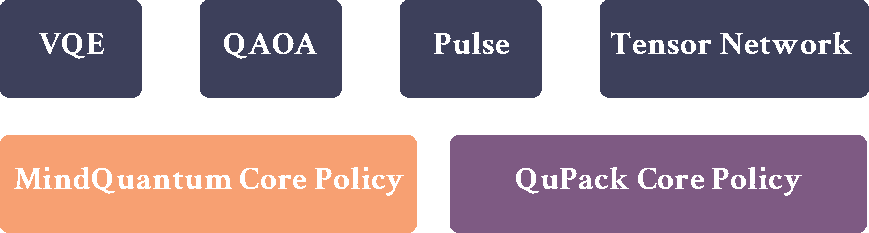
\includegraphics[scale=0.5]{./images/6_qupack_layer.pdf}
    \captionsetup{justification=raggedright,singlelinecheck=false}
    \caption{\label{6_qupack_layer} The structure of \QuPack. Based on core simulation policy in \MindQuantum\ and specific designed policy in \QuPack, we are able to build high performance application like VQE, QAOA, Pulse and Tensor Network simulator.}
\end{figure}
